\documentclass[preprint,12pt]{elsarticle}
\usepackage[T1]{fontenc}
\usepackage[utf8]{inputenc}
\usepackage{lmodern}
\usepackage{microtype}
\usepackage{graphicx}
\usepackage{booktabs}
\usepackage{array}
\usepackage{tabularx}
\usepackage{amsmath,amssymb}
\usepackage{enumitem}
\usepackage{float}
\usepackage{placeins}
\usepackage{xurl}
\usepackage[hidelinks]{hyperref}
\setlength{\emergencystretch}{3em}
\newcolumntype{L}[1]{>{\raggedright\arraybackslash}p{#1}}
\makeatletter
\setlength{\@fptop}{0pt}
\makeatother
\journal{Smart Agricultural Technology}
% Author metadata supplied by the author team on 2026-08-11.
\newif\ifAuthorMetadataReady
\AuthorMetadataReadytrue

\newcommand{\CorrespondingAuthor}{Zhuo Chen}
\newcommand{\CorrespondingEmail}{zhuoc@chalmers.se}
\newcommand{\CorrespondingAffiliation}{Chalmers University of Technology, SE-412 96 Gothenburg, Sweden}

\newcommand{\AuthorFrontmatter}{%
  \def\thefnote{$\dagger$}%
  \author[aff-a]{Shuhao Liu\fnref{equal}}
  \ead{2420610137@stu.hrbust.edu.cn}
  \author[aff-b]{Zhuo Chen\fnref{equal}\corref{corresponding}}
  \ead{zhuoc@chalmers.se}
  \author[aff-c]{Zhi Ling}
  \ead{zhi.ling@kiwiar.com}
  \author[aff-c]{Yu Yan}
  \ead{yu.yan@kiwiar.com}
  \author[aff-a]{Jie Liu}
  \ead{liujie@hrbust.edu.cn}
  \author[aff-a]{Qiuxue Wu}
  \ead{2420610140@stu.hrbust.edu.cn}
  \author[aff-c]{Ziyi Kuang}
  \ead{ziyi.kuang@kiwiar.com}
  \address[aff-a]{Harbin University of Science and Technology, No. 52 Xuefu Road, Nangang District, Harbin 150080, Heilongjiang, China}
  \address[aff-b]{Chalmers University of Technology, SE-412 96 Gothenburg, Sweden}
  \address[aff-c]{Kiwiar Co., Ltd., Singapore}
  \fntext[equal]{These authors contributed equally to this work.}
  \cortext[corresponding]{Corresponding author.}
}

% These statements require separate confirmation from the author team.
\newif\ifFundingStatementReady
\FundingStatementReadyfalse
\newcommand{\FundingStatement}{}
\newif\ifCompetingInterestsReady
\CompetingInterestsReadyfalse
\newcommand{\CompetingInterests}{}
\newif\ifCRediTStatementReady
\CRediTStatementReadyfalse
\newcommand{\CRediTStatement}{}
\newcommand{\RepositoryDOI}{}


\begin{document}
\begin{frontmatter}

\title{From Candidate Scores to Plant Recovery in Finite Crop--Weed Review Queues}
\ifAuthorMetadataReady
\AuthorFrontmatter
\else
\author{Anonymous manuscript}
\address{Author identities and affiliations are withheld for blinded review.}
\fi

\begin{abstract}
Crop--weed models are commonly evaluated at pixel or candidate level, although a finite review queue succeeds only when distinct plants remain represented after proposal formation, role qualification, ranking, and budget truncation. We formulate an instance-support-aware evaluation that separates these losses and uses deterministic one-to-one matching as its primary endpoint. The framework was evaluated on the official WeedsGalore split (104/26/26 RGB tiles) and in a locked cross-dataset test on 60 CWFID images. At a common 471-candidate test budget, proposal commissioning increased one-to-one role-qualified weed recall from 0.0970 to 0.1157; the paired image-bootstrap difference was 0.0187 (95\% CI 0.0032--0.0347). Under fixed $K=20$ queues, Mask R-CNN reached one-to-one recall 0.2159, compared with 0.2027 for a ResNet-18 U-Net; validation-selected semantic-probability ordering reached 0.2117. Two independent operators agreed on weed reviewability for 94.2\% of 518 queued regions ($\kappa=0.893$). The locked CWFID transfer produced no candidates from any of five WeedsGalore-selected checkpoints, despite stable internal results. Instance-support-aware accounting therefore distinguishes improvements in recoverable plant support from improvements in candidate scores, while exposing threshold-transfer failures that internal validation cannot reveal.
\end{abstract}

\begin{keyword}
crop--weed segmentation \sep instance matching \sep review queue \sep review budget \sep cross-dataset evaluation \sep precision agriculture
\end{keyword}
\end{frontmatter}

\section{Introduction}

Site-specific weed management connects sensing, plant localisation, crop--weed discrimination, and intervention \cite{slaughter2008robotic,swinton2005economics}. Segmentation quality is usually summarised by pixel overlap, while instance systems are commonly evaluated by average precision. These metrics describe model output, but they do not establish how many distinct plants remain available to a reviewer when only a finite number of regions can be inspected.

Finite review introduces a sequence of losses. A plant can be absent from the proposal pool, contained in a mixed crop--weed region, merged with neighbouring plants, ranked below the review cut-off, or duplicated by several candidates. Object-proposal research relates recall to overlap and proposal count \cite{hosang2016proposals}, and precision-at-the-top learning studies ranking under restricted capacity \cite{kar2015precision}. Neither candidate discrimination nor many-to-one coverage alone resolves duplication and merge effects. A plant-level queue therefore requires an explicit matching contract between selected regions and distinct truth instances.

The queue studied here is a post-inference tool for offline agronomic quality assurance and annotation triage. A reviewer may retain a region as weed evidence, reject it, or escalate an ambiguous crop--weed mixture. Crop overlap matters because it identifies regions that require additional scrutiny before they enter an annotation or quality-control record; it is not interpreted as an agronomic treatment risk. This differs from active learning, which chooses observations for model annotation or retraining \cite{sheikh2020gradient,vanmarrewijk2024active}; selective prediction, which abstains from automated outputs \cite{geifman2017selective,geifman2019selectivenet}; and learning to defer, which learns assignment between a model and an expert \cite{mozannar2020defer,mozannar2023whoshould}. The present queue orders already generated regions and does not issue an actuation decision.

Agricultural imagery adds spatial, temporal, and cross-dataset dependence. Random image partitions can overstate generalisation when neighbouring observations share soil, illumination, canopy structure, or management \cite{roberts2017spatial}. Public crop--weed datasets also differ in crop, sensor, viewpoint, scale, and annotation contract \cite{haug2015cwfid,chebrolu2017sugarbeets,steininger2023cropandweed,weyler2024phenobench,celikkan2025weedsgalore}. Internal optimisation stability must therefore be separated from transfer across acquisition systems.

We address this gap through an instance-support-aware evaluation of finite crop--weed review queues. The framework distinguishes spatial proposal recall, role-qualified proposal recall, and queued one-to-one plant recovery. It also matches review burden when proposal settings are compared, discloses every source of supervision, and treats candidate AUC and average precision as diagnostic measures. We evaluate source-transfer rankers, target-trained semantic models, an instance segmenter, and simple probability or entropy ordering under the same $K=20$ capacity. A frozen CWFID protocol then tests whether validation-selected WeedsGalore checkpoints and thresholds transfer without external tuning. The resulting analysis identifies where recoverable support is gained, where it is lost, and when an internally stable queue fails across datasets.

\section{Materials and methods}

\subsection{Review task and information contract}

The unit presented for review was an RGB region associated with one connected proposal component and a model score. Each tile contributed at most $K=20$ regions. The value $K=20$ defines a standardised experimental capacity; it is not a measured time optimum or a per-hectare workload. The intended reviewer action is retain, reject, or escalate. No autonomous treatment command, operator timing, or labour-cost claim is evaluated.

Figure~\ref{fig:workflow} separates model input from offline scoring. Queue construction can use RGB, model outputs, component geometry, tile identity, and a preselected policy. Target truth can enter training, validation selection, or offline scoring only in its declared data role. Test masks and instance identifiers cannot enter proposal generation, ranking features, or queue allocation.

Taxonomic identity, agricultural role, and management morphotype are distinct output axes. Family, genus, and species form the taxonomic axis. Crop, weed, volunteer crop, and unknown role are scene-dependent agricultural roles. Grass-like, broadleaf, sedge, and other describe management morphotype. The experiments in this paper evaluate only the crop--weed role axis.

\begin{figure}[!t]
\centering
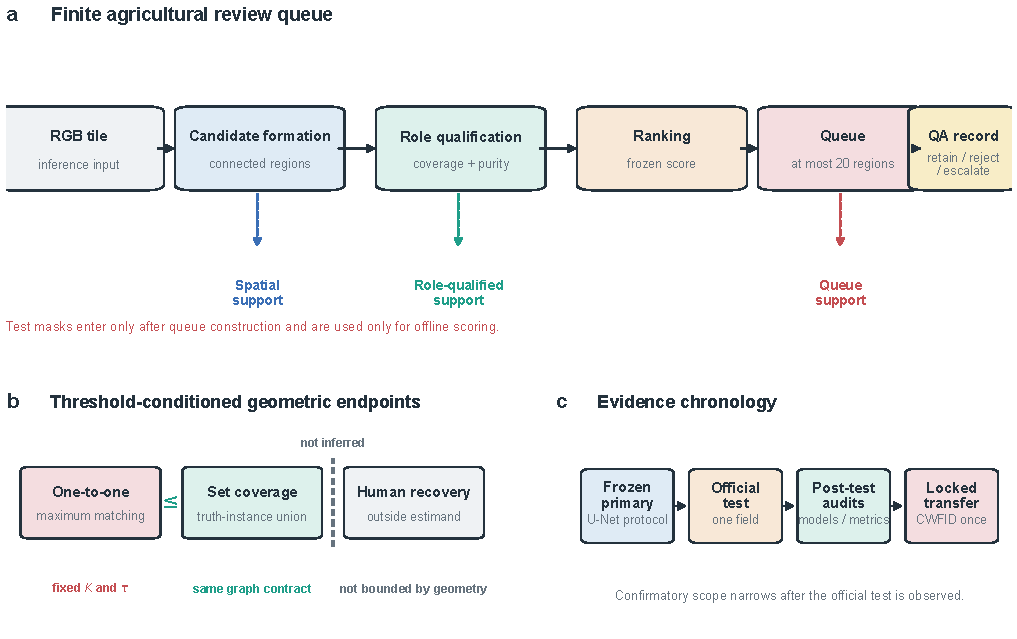
\includegraphics[width=\textwidth]{figures/Figure_1.pdf}
\caption{Instance-support-aware evaluation of a finite crop--weed review queue. RGB images pass through candidate formation, role scoring, ranking, and a fixed $K=20$ budget. Offline truth first measures spatial support, then role-qualified support, and finally deterministic one-to-one plant recovery. Training and validation truth remain separated from locked test scoring. The external branch transfers WeedsGalore-selected checkpoints and thresholds to CWFID without external tuning.}
\label{fig:workflow}
\end{figure}

\subsection{Datasets, splits, and external lock}

The source specialists used public SugarBeets2016 RGB images and masks \cite{chebrolu2017sugarbeets}. The target development study used 156 annotated $600\times600$ pixel WeedsGalore tiles from one maize field \cite{celikkan2025weedsgalore}. The official spatial allocation contains 104 training, 26 validation, and 26 test tiles. Raster enumeration yielded 2,168 crop and 10,029 weed instances across all 156 tiles. The official test masks contained 256 crop and 1,712 weed instances.

The test tiles represented four acquisition dates (Table~\ref{tab:dates}). The first three dates contributed eight tiles each, whereas 15 June contributed two. Date-macro and worst-date summaries therefore complement pooled counts. Capture-index groups are reported as released grouping variables, without assigning unverified physical field identities.

\begin{table}[!t]
\centering
\caption{WeedsGalore official-test denominators by acquisition date.}
\label{tab:dates}
\small
\begin{tabular}{lrrr}
\toprule
Acquisition date & RGB tiles & Weed instances & Crop instances \\
\midrule
25 May 2023 & 8 & 392 & 122 \\
30 May 2023 & 8 & 440 & 55 \\
6 June 2023 & 8 & 726 & 68 \\
15 June 2023 & 2 & 154 & 11 \\
\midrule
Total & 26 & 1,712 & 256 \\
\bottomrule
\end{tabular}
\end{table}

Cross-dataset evaluation used the official CWFID v1.0 release \cite{haug2015cwfid}. Its 60 RGB images and paired public annotations were fixed at source commit \texttt{176612f3}. Before image or annotation access, the protocol fixed preprocessing, five existing WeedsGalore checkpoints, their validation-selected component settings, fixed $K=20$, the ranking score, truth-component definition, and endpoints. All 242 upstream blobs were verified by byte count and Git blob SHA-1 before one recorded opening. Images were scaled so the longer side measured 600 pixels, reflection-padded to $600\times600$, and normalised as in training. Public annotation colours were transformed by nearest-neighbour interpolation and zero padding. Weed truth units were eight-connected annotation components of at least 16 pixels; they are component proxies rather than persistent plant identities. No CWFID label was used for fitting or selection.

\subsection{Supervision ledger}

Table~\ref{tab:supervision} reports the complete supervision burden. Proposal generation itself is image-only at inference, but selecting its operating point requires target-training masks. Candidate labels are derived from dense masks. A separate 300-candidate training-label ablation therefore restricts sampled training candidates while retaining all 2,436 labelled validation candidates; it is not a 300-label end-to-end regime.

\begin{table}[!t]
\centering
\caption{Supervision and data roles. Test truth is restricted to offline scoring.}
\label{tab:supervision}
\footnotesize
\setlength{\tabcolsep}{3.5pt}
\begin{tabularx}{\textwidth}{L{3.2cm}L{3.2cm}L{3.4cm}X}
\toprule
System or stage & Training supervision & Selection supervision & Test use \\
\midrule
Source specialists & 7,050 SugarBeets RGB masks & 901 source masks for diagnostics & RGB inference only \\
Proposal commissioning & 104 target dense masks & Training-mask objective and burden constraint & Offline scoring \\
Source-transfer rankers & 9,887 target-training candidate labels & 2,436 validation candidate labels & Queue formed before scoring \\
U-Net and DeepLabV3+ & 104 target RGB dense masks & 26 validation RGB dense masks & Queue formed before scoring \\
Mask R-CNN & 104 target RGB semantic and instance masks & 26 validation semantic and instance masks & Queue formed before scoring \\
CWFID transfer & No external labels & No external labels & 60 annotations for locked scoring only \\
Two-operator review & No model training & Frozen 518-region queue and common instructions & Aggregate technical-review analysis only \\
\bottomrule
\end{tabularx}
\end{table}

\subsection{Two-operator technical review}

A frozen target-semantic $K=20$ queue containing 518 regions from the 26 WeedsGalore test tiles was used to assess whether the review categories could be applied consistently. Each item showed the RGB tile, a highlighted candidate box, and a local RGB crop. Acquisition date, scene identity, candidate identifier, model score, rank, model identity, allocation policy, and mask-derived truth were hidden. Two operators completed all items independently under common written instructions and without access to one another's responses.

For each region, the operators recorded primary content (weed-dominant, crop-dominant, background, or uncertain), weed reviewability (yes, no, or uncertain), crop presence (yes, no, or uncertain), localisation usability (adequate, partial, unusable, or uncertain), and confidence on a five-point scale. Timing was neither required nor analysed. Exact agreement and Cohen's $\kappa$ were computed for the categorical fields. A 10,000-replicate scene-cluster bootstrap resampled the 26 source tiles. The analysis characterises these two fixed operators and was not used to select a model, threshold, or queue policy.

\subsection{Candidate formation and model families}

Two source ResNet-18 U-Net-style specialists were initialised with ImageNet-1K weights \cite{he2016resnet}. One estimated plant foreground and the other estimated crop and weed role probabilities. The source-training procedures used deterministic $128\times128$ patches, AdamW, and combined cross-entropy and soft-Dice losses. Full hyperparameters and source diagnostics are reported in the supplement. A target tile produced foreground probability $f(u)$ and role probabilities $p_c(u)$ and $p_w(u)$. Thresholding $f(u)$ at $T$, applying eight-connectivity, and removing components smaller than $A$ pixels defined each proposal setting $(T,A)$.

The original operating point was $(0.95,32)$. Commissioning searched 12 settings on the 104 official-training tiles. Feasible settings had no more than 100 candidates per tile on average. Training role-qualified weed proposal recall was maximised, followed by lower burden, higher threshold, and larger area. The selected setting was $(0.70,32)$.

Five all-candidate rankers were evaluated: the source weed score, geometry, role-plus-local specialist features, frozen DINOv2 ViT-S/14 features, and component-masked DINOv2 features \cite{oquab2024dinov2}. The masked view retained component pixels and filled the surrounding bounding box with the image median. Logistic regularisation was selected on official validation. The target-trained semantic family comprised a ResNet-18 U-Net and DeepLabV3+ with a ResNet-50 encoder \cite{chen2018deeplabv3plus}. The instance family used Mask R-CNN with a ResNet-50 FPN backbone \cite{he2017maskrcnn}. U-Net used five training seeds; DeepLabV3+ and Mask R-CNN used three each. Each seed selected its epoch and component setting on the official validation split.

Semantic components were ranked by conditional weed probability, mean weed probability, or mean predictive entropy. The policy for each checkpoint was selected on validation by one-to-one role-qualified recall, then candidate precision, then policy name. Mask R-CNN ranked predicted weed instances before other detections and then used detection confidence. All model families used the same fixed $K=20$ queue endpoint. Training ran on one NVIDIA H200 accelerator per seed; hardware details, exact software versions, public-weight hashes, and checkpoint hashes are provided in the reproducibility archive.

\subsection{Support, matching, and queue metrics}

For truth instance $I_j$ and candidate $C_i$, instance coverage is
\begin{equation}
\operatorname{cov}(I_j,C_i)=\frac{|I_j\cap C_i|}{|I_j|}.
\end{equation}
Spatial proposal recall counts $I_j$ when at least one candidate has coverage of 0.50 or greater. Role-qualified support additionally requires the candidate to contain at least 0.50 labelled-pixel coverage and 0.90 same-role purity. These thresholds define an offline matching contract rather than an agronomic treatment threshold.

Many-to-one recall permits one candidate to recover several truth instances. The primary endpoint instead uses maximum-cardinality one-to-one matching between selected candidates and weed instances that satisfy the role-qualified contract. Lexicographic candidate and instance identifiers resolve deterministic ties. Candidate precision is the fraction of selected regions that satisfy the role-qualified weed contract. Crop exposure is the fraction of tiles with any selected region overlapping crop truth. Standard IoU and threshold sensitivity are reported separately.

\subsection{Matched review burden and uncertainty}

Commissioning changes both proposal support and candidate burden. To isolate formation quality at a common review burden, the paired comparison used
\begin{equation}
k_i=\min(20,n_i^{\mathrm{original}},n_i^{\mathrm{commissioned}})
\end{equation}
for each test tile $i$. Both settings therefore contributed the same 471 selected candidates under identical ranker weights. A global equal-$N$ analysis also ranked 471 candidates for each setting. Recall--burden curves for $K\in\{1,5,10,20,50\}$ were summarised by their normalised area (AURBC).

Uncertainty was estimated with 10,000 paired bootstrap resamples of the 26 test images. Training-seed means and sample standard deviations quantify optimisation variation. Image-cluster percentile intervals quantify test-image heterogeneity. Two prespecified strong-baseline contrasts compare DeepLabV3+ and Mask R-CNN with the ResNet-18 U-Net. Candidate AUC and average precision are diagnostic and are not treated as plant-recovery endpoints. The provenance class of each analysis and the recorded freeze and opening times for the external experiment are reported in Supplementary Table~S1.

\section{Results}

\subsection{Commissioning improved recovery under a matched review burden}

Before budget matching, the original setting produced 802 candidates (30.85 per tile), while the commissioned setting produced 2,351 (90.42 per tile). Spatial proposal recall increased from 509/1,712 (0.2973) to 978/1,712 (0.5713). Role-qualified proposal recall increased from 330/1,712 (0.1928) to 518/1,712 (0.3026).

The gain remained after review burden was matched (Table~\ref{tab:commissioning}). Both settings selected 471 candidates. One-to-one role-qualified recall increased from 0.0970 to 0.1157, a paired difference of 0.0187 (95\% image-bootstrap CI 0.0032--0.0347). Spatial recall increased by 0.0818 (95\% CI 0.0560--0.1098). Candidate precision decreased by 0.0679 (95\% CI $-0.1384$--0.0064), and crop-exposed tile frequency increased by 0.0385 (95\% CI 0--0.1154). Under global equal-$N$, one-to-one recall increased from 0.0970 to 0.1174. AURBC increased from 0.0598 to 0.0750. Commissioning therefore added recoverable support, but also introduced more ambiguous regions and crop overlap.

\begin{table}[!t]
\centering
\caption{Proposal settings compared at the same 471-candidate review burden. Recall denominators are 1,712 weed instances; crop exposure denominators are 26 tiles.}
\label{tab:commissioning}
\footnotesize
\setlength{\tabcolsep}{3pt}
\resizebox{\textwidth}{!}{%
\begin{tabular}{lrrrrrr}
\toprule
Setting & Raw candidates/tile & Selected & Precision & Spatial recall & Qualified recall & 1:1 recall \\
\midrule
Original $(0.95,32)$ & 30.85 & 471 & 0.5860 & 0.1875 & 0.1197 & 0.0970 \\
Commissioned $(0.70,32)$ & 90.42 & 471 & 0.5180 & 0.2693 & 0.1571 & \textbf{0.1157} \\
\bottomrule
\end{tabular}}
\end{table}

\begin{figure}[!t]
\centering
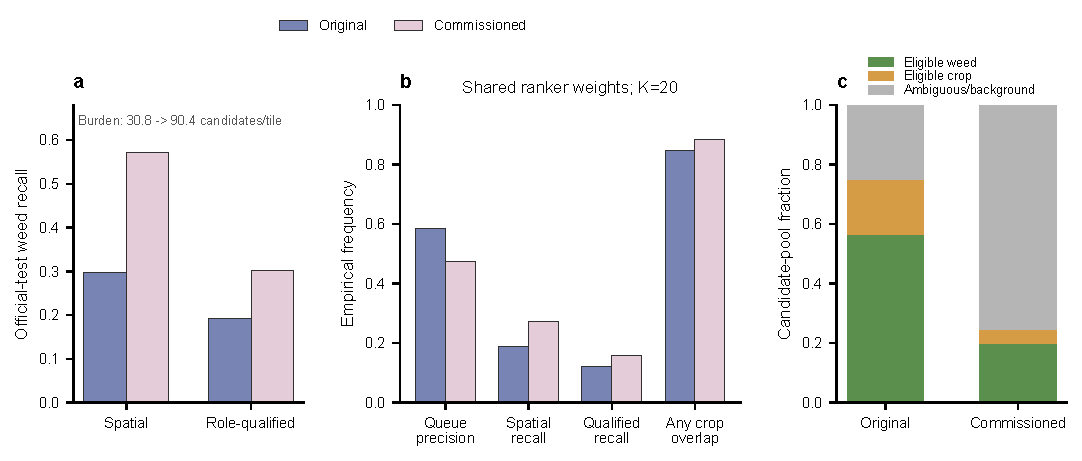
\includegraphics[width=\textwidth]{figures/Figure_2.pdf}
\caption{Matched-burden commissioning analysis. (a) Raw proposal recall and candidate burden. (b) Original and commissioned queues after applying a common per-tile capacity, with 95\% image-bootstrap intervals. (c) Paired commissioned-minus-original effects. (d) One-to-one recall--burden curves and normalised AURBC.}
\label{fig:commissioning}
\end{figure}

\subsection{Candidate discrimination did not determine plant recovery}

Changing the fitting target from eligible candidates to the complete deployed candidate pool increased role-plus-local candidate AUC from 0.4420 to 0.9049. Frozen DINOv2 reached AUC/AP of 0.9630/0.8684, while component masking reached 0.9665/0.8813. The absolute masking differences were 0.0035 in AUC and 0.0129 in AP.

High candidate discrimination did not translate directly to distinct-plant recovery. At $K=20$, the masked DINOv2 queue achieved candidate precision 0.5346 and many-to-one qualified recall 0.1863. One-to-one matching reduced recall to 0.1343 because merged candidates and duplicate support could not be counted repeatedly. The role-qualified proposal ceiling was 0.3026, and an exact per-tile budget oracle reached 0.2488. Proposal formation therefore removed most plants before ranking, while candidate multiplicity created an additional gap between many-to-one and one-to-one evaluation.

The qualitative atlas in Figure~\ref{fig:failures} shows four mechanisms selected deterministically from the 26 test tiles: fragmentation of one weed into two candidates, merger of five weeds into one candidate, a background component with no labelled support, and a crop--weed mixture. Each mechanism changes plant recovery without being fully described by a single candidate score.

\begin{figure}[!t]
\centering
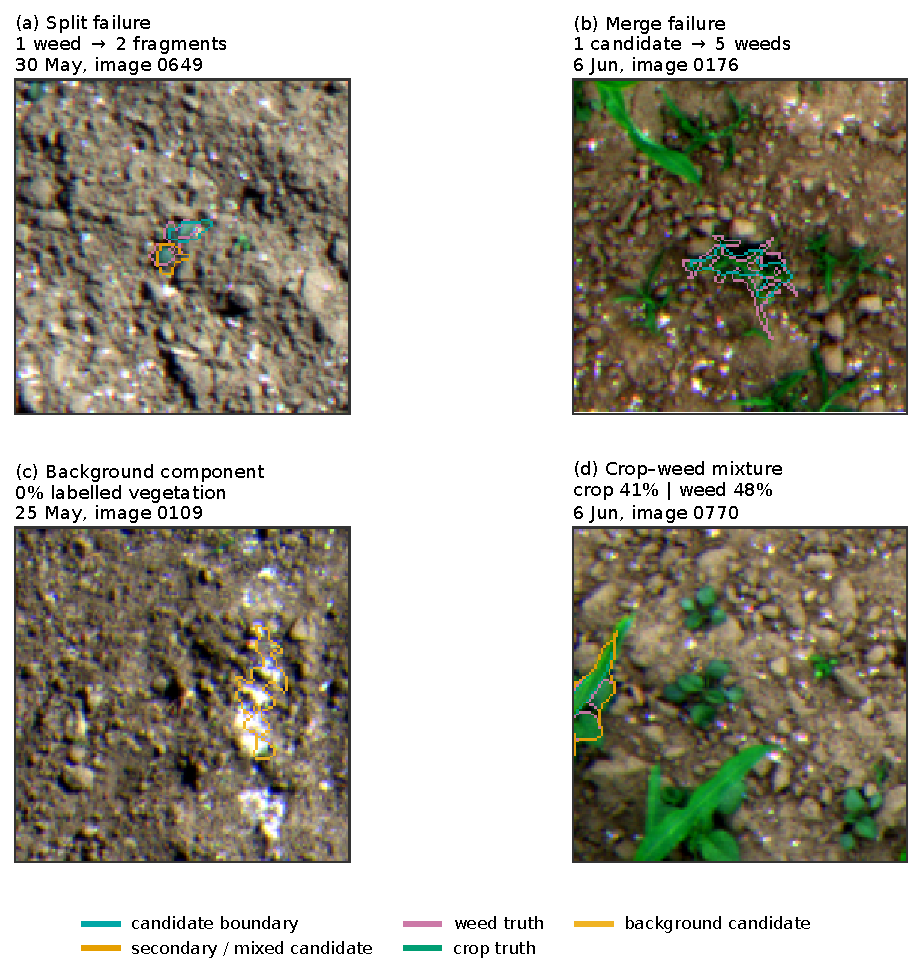
\includegraphics[width=\textwidth]{figures/Figure_4.pdf}
\caption{Instance-support failure atlas from WeedsGalore test tiles. Coloured contours show proposal components and truth support. (a) One weed split into two fragments. (b) One candidate merged five weed instances. (c) A background-dominated component contained no labelled plant pixels. (d) A mixed component contained both crop and weed support. Selection rules and source identifiers are provided in the source-data table.}
\label{fig:failures}
\end{figure}

\subsection{Strong baselines changed the ordering of queue systems}

Under the same $K=20$ contract, Mask R-CNN achieved the highest one-to-one recall and candidate precision (Table~\ref{tab:strong}). Its mean one-to-one recall was 0.2159 across three seeds, compared with 0.2027 across five U-Net seeds. The paired image-bootstrap contrast was 0.0132 (95\% CI 0.0015--0.0284). DeepLabV3+ reached 0.1924; its contrast with U-Net was $-0.0103$ (95\% CI $-0.0216$ to $-0.0002$). Mask R-CNN simultaneously reduced many-to-one spatial recall relative to U-Net by 0.0254 (95\% CI $-0.0485$ to $-0.0015$), illustrating that candidate compactness and one-to-one separability favour different endpoints.

Validation selected mean weed probability for four U-Net seeds and conditional weed probability for one. These simple semantic scores achieved one-to-one recall $0.2117\pm0.0047$ and precision $0.7440\pm0.0185$. Their queue recall was close to Mask R-CNN and above the default U-Net score. Predictive entropy was evaluated within the same candidate pool but was not selected. The internal comparison therefore supports explicit plant matching and model-family choice, rather than added feature complexity, as the main determinants of queue performance.

\begin{table}[!t]
\centering
\caption{Fixed $K=20$ WeedsGalore queues. Values are mean $\pm$ sample SD across independently trained seeds. The probability row reorders the five U-Net component pools using validation-selected semantic scores.}
\label{tab:strong}
\footnotesize
\setlength{\tabcolsep}{3pt}
\resizebox{\textwidth}{!}{%
\begin{tabular}{lrrrrrr}
\toprule
System & Seeds & Precision & Spatial recall & Qualified recall & 1:1 recall & Crop-exposed tiles \\
\midrule
ResNet-18 U-Net & 5 & $0.7168\pm0.0260$ & $0.2668\pm0.0211$ & $0.2468\pm0.0231$ & $0.2027\pm0.0057$ & $0.2462\pm0.0439$ \\
DeepLabV3+--ResNet-50 & 3 & $0.6832\pm0.0042$ & $0.2710\pm0.0107$ & $0.2420\pm0.0094$ & $0.1924\pm0.0032$ & $0.2436\pm0.0222$ \\
Mask R-CNN--ResNet-50-FPN & 3 & $\mathbf{0.7891\pm0.0142}$ & $0.2414\pm0.0041$ & $0.2259\pm0.0053$ & $\mathbf{0.2159\pm0.0038}$ & $0.2308\pm0.0769$ \\
Validation-selected probability ranking & 5 & $0.7440\pm0.0185$ & $\mathbf{0.3391\pm0.0249}$ & $\mathbf{0.2873\pm0.0082}$ & $0.2117\pm0.0047$ & $0.2846\pm0.0516$ \\
\bottomrule
\end{tabular}}
\end{table}

\begin{figure}[!t]
\centering
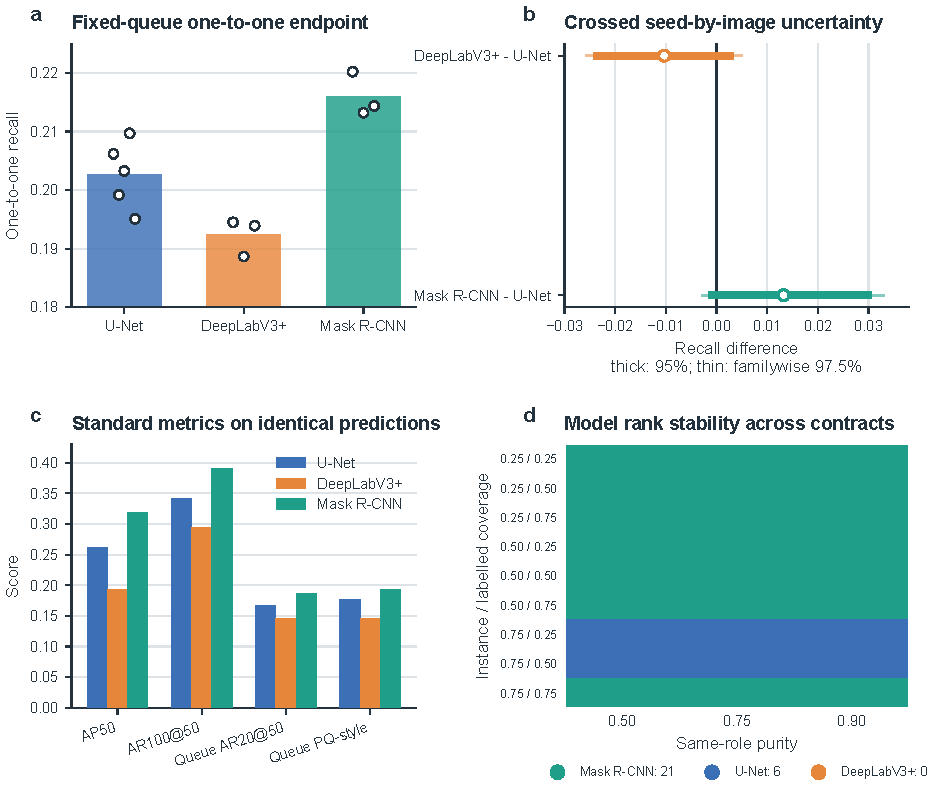
\includegraphics[width=\textwidth]{figures/Figure_3.pdf}
\caption{Strong-baseline comparison on the 26 WeedsGalore test tiles. (a) Candidate precision and (b) one-to-one role-qualified recall; bars show seed means and points show individual seeds. (c) Paired image-bootstrap contrasts with the ResNet-18 U-Net. (d) U-Net one-to-one recall by acquisition date, with tile and weed-instance denominators shown above each group.}
\label{fig:strong}
\end{figure}

Internal performance varied by acquisition date. The five U-Net seeds achieved mean one-to-one recall of 0.1378, 0.2864, 0.2061, and 0.1130 on 25 May, 30 May, 6 June, and 15 June, respectively. Corresponding precision was 0.4035, 0.8163, 0.9513, and 0.5650. The 15 June estimate represents only two tiles and 154 weed instances. Pooled performance therefore combines materially different date-specific conditions.

\subsection{Independent operators applied the review categories consistently}

Both operators completed all 518 queued regions. They agreed on weed reviewability for 488 regions (0.9421), with Cohen's $\kappa=0.8930$ (Table~\ref{tab:operators}). The scene-cluster bootstrap interval was 0.9228--0.9611 for exact agreement and 0.8474--0.9249 for $\kappa$. Both marked 301 regions as reviewable weed evidence and 143 as not reviewable; 74 were disputed or included at least one uncertain response. Agreement exceeded 0.94 for primary content, crop presence, and localisation usability.

Of the 301 consensus-reviewable regions, 249 also satisfied the mask-derived role-qualified weed contract (0.8272). Human reviewability and geometric mask qualification therefore overlapped strongly but were not equivalent: a reviewer can recognise useful weed evidence in a partial or mixed crop, while the offline contract applies fixed coverage and purity thresholds.

\begin{table}[!t]
\centering
\caption{Agreement between two independent operators on the frozen 518-region review queue.}
\label{tab:operators}
\small
\begin{tabular}{lrr}
\toprule
Review field & Exact agreement & Cohen's $\kappa$ \\
\midrule
Primary content & 0.9479 & 0.9095 \\
Weed reviewability & 0.9421 & 0.8930 \\
Crop presence & 0.9459 & 0.8492 \\
Localisation usability & 0.9402 & 0.9049 \\
\bottomrule
\end{tabular}
\end{table}

\subsection{Locked cross-dataset evaluation exposed complete threshold-transfer failure}

The CWFID lock was opened once after all 242 upstream blobs, five checkpoint hashes, and 60 RGB--annotation pairs passed audit. The primary truth definition yielded 331 weed components across 60 images. Every WeedsGalore-selected checkpoint classified all CWFID pixels as background at its frozen operating point. Consequently, all five seeds generated zero candidates, selected zero regions, and recovered zero weed components. One-to-one role-qualified recall was 0 with an image-bootstrap 95\% interval of 0--0. Weed and crop IoU were both 0; background IoU was 0.9450.

The identical result across five checkpoints separates optimisation stability from acquisition transfer. The internal U-Net queue varied only from 0.1951 to 0.2097 in one-to-one recall, yet none of those validation-selected component thresholds transferred to CWFID. This outcome rules out a cross-dataset performance claim for the present queue and identifies component calibration as a prerequisite for deployment beyond the development dataset.

\begin{figure}[!t]
\centering
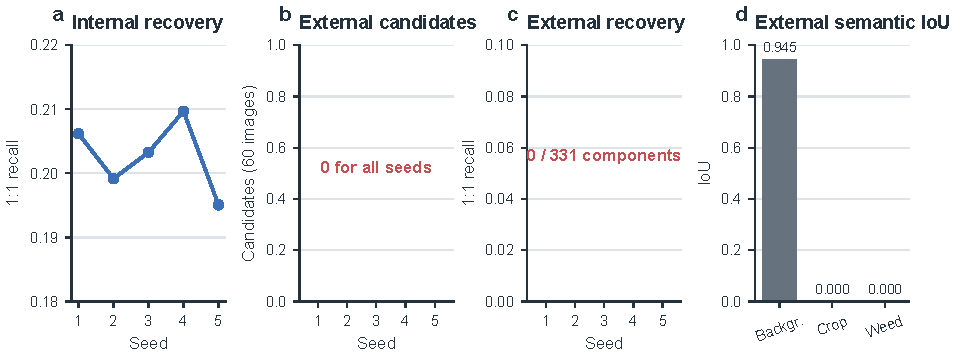
\includegraphics[width=\textwidth]{figures/Figure_5.pdf}
\caption{Locked CWFID transfer without external tuning. (a) WeedsGalore fixed-queue one-to-one recall across five U-Net seeds. (b) CWFID candidate burden for the same checkpoints. (c) CWFID weed-component recovery. (d) CWFID semantic IoU. All 60 images and 331 weed components contributed to every external seed result.}
\label{fig:external}
\end{figure}

\section{Discussion}

Instance-support-aware evaluation changes how a crop--weed queue is judged. Candidate AUC described ordering inside a generated pool, whereas one-to-one recall measured whether distinct plants survived the full proposal-to-budget chain. The difference was substantial: the masked DINOv2 ranker reached candidate AUC 0.9665, yet recovered 0.1343 of weed instances under one-to-one matching. Direct target-trained models recovered approximately 0.19--0.22 under the same budget. Candidate scores and plant recovery are therefore related but non-interchangeable evidence levels.

The burden-matched commissioning analysis isolates a genuine proposal effect. Lowering the foreground threshold increased raw candidate burden almost threefold, but the commissioned pool still recovered more plants when both settings were restricted to 471 reviews. The gain was modest in absolute terms and accompanied by lower precision and greater crop exposure. Recall--burden curves provide a weight-free way to represent this trade-off without assigning an arbitrary utility to a recovered weed, an ambiguous region, or a crop overlap.

Strong baselines refine the technical conclusion. Mask R-CNN provided the highest internal one-to-one recall and precision, while DeepLabV3+ did not improve on the smaller U-Net for the queue endpoint. A simple validation-selected semantic-probability score nearly matched Mask R-CNN. Frozen DINOv2 remained useful as a diagnostic ranker, but its small masking ablation and lower one-to-one recovery do not establish a need for an additional representation stage. The reusable contribution is the evaluation contract that exposes support, multiplicity, and review burden across model families.

The two-operator study shows that the queue categories are interpretable in a concrete review setting. High agreement coexisted with a measurable difference between consensus reviewability and the mask-derived contract, supporting separate reporting of human decisions and geometric matching. The study records category consistency rather than operator-population performance or labour cost; review-time and area-normalised workload remain separate evaluation targets.

The locked CWFID result defines the transfer boundary directly. Five internally stable checkpoints produced the same all-background outcome on a different crop, camera geometry, image scale, and acquisition distribution. Because no external label changed a threshold, the result measures the frozen system rather than a retuned variant. Cross-dataset calibration or unsupervised operating-point adaptation is therefore a separate technical problem. It cannot be inferred from seed stability within one field.

The intended queue supports offline image quality assurance and annotation triage. A region can be retained, rejected, or escalated, and the finite budget makes omissions auditable. The current evidence does not measure operator time or agronomic treatment value, so $K=20$ should be read as a controlled capacity unit. WeedsGalore supplies multitemporal internal evidence from one maize field; CWFID supplies an independently acquired carrot-field stress test but uses connected components rather than persistent plant identities. Evaluation across additional farms, seasons, sensors, and reviewer workflows is needed to relate plant recovery to operational cost.

\section{Conclusion}

This study establishes an instance-support-aware evaluation for finite crop--weed review queues. Matched-burden analysis showed that proposal commissioning increased recoverable plant support, strong baselines identified Mask R-CNN and simple semantic-probability ordering as effective internal systems, and independent operators applied the review categories consistently. The locked CWFID test then exposed complete failure of the transferred component thresholds. Separating spatial support, role qualification, one-to-one matching, human reviewability, and review capacity makes both internal improvements and cross-dataset failures visible before a queue is assigned operational meaning.

\section*{Data availability}
SugarBeets2016, WeedsGalore, and CWFID are public datasets available from their cited official sources. The reproducibility archive records source URLs, access dates, release identifiers, licence information, exact source revisions, and integrity hashes. Public imagery remains with the original repositories. Derived source-data tables, result manifests, and verification hashes accompany the code release.

\section*{Code availability}
The versioned reproducibility materials are maintained at \url{https://github.com/Fytap/agrispec-vlm-reproducibility}. The release contains frozen configurations, environment specifications, model acquisition records, training and evaluation source, archived predictions and matching outputs, source tables for every figure, failure records, and clean-room replay commands. Public dataset imagery and public model weights remain at their upstream sources.

\section*{Declaration of Generative AI and AI-Assisted Technologies in the Manuscript Preparation Process}
During the preparation of this work, the authors used OpenAI Codex for code review, reproducibility checks, and language editing, including checks of sentence clarity, grammar, and wording. The authors reviewed and edited all affected content and take full responsibility for the content of the publication.

\section*{Ethics declaration}
This study analysed public agricultural image datasets. Two operators performed technical quality assurance on model-generated agricultural image regions; no personal, sensitive, demographic, or behavioural data were collected, and no operator identity is reported. This annotation and software-quality activity did not constitute human-subject research and did not require formal ethical approval. No animals were involved.

\section*{Declaration of competing interest}
Zhi Ling, Yu Yan, and Ziyi Kuang report an affiliation with Kiwiar Co., Ltd. No proprietary dataset or commercial product was evaluated in this study.

\ifFundingStatementReady
\section*{Funding}
\FundingStatement
\fi

\ifCRediTStatementReady
\section*{CRediT authorship contribution statement}
\CRediTStatement
\fi

\setlength{\bibsep}{0pt}
\small
\bibliographystyle{elsarticle-num}
\bibliography{references}

\end{document}
